\documentclass[pdftex,12pt,a4paper]{article}
\pdfpagewidth 8.5in
\pdfpageheight 11.6in
\linespread{1.3}
\usepackage{anysize}
\marginsize{2.5cm}{2.5cm}{2.5cm}{2.5cm}

\usepackage[utf8]{inputenc}
\usepackage[T1]{fontenc}
\usepackage[magyar]{babel}
\usepackage{indentfirst}
\usepackage{amsmath}
\usepackage{float}
\usepackage{graphicx}
\usepackage{braket}
\usepackage[unicode,pdftex]{hyperref}
\usepackage{hyperref}
\usepackage{breqn}

\usepackage{listings}
\usepackage{xcolor}

\definecolor{codegreen}{rgb}{0,0.6,0}
\definecolor{codegray}{rgb}{0.3,0.3,0.3}
\definecolor{codepurple}{rgb}{0.58,0,0.82}
\definecolor{backcolour}{rgb}{0.90,0.90,0.87}

\lstdefinestyle{mystyle}{
    backgroundcolor=\color{backcolour},   
    commentstyle=\color{codegreen},
    keywordstyle=\color{magenta},
    numberstyle=\small\color{codegray},
    stringstyle=\color{codepurple},
    basicstyle=\ttfamily\small,
    breakatwhitespace=false,         
    breaklines=true,                 
    captionpos=b,                    
    keepspaces=true,                 
    numbers=left,                    
    numbersep=5pt,                  
    showspaces=false,                
    showstringspaces=false,
    showtabs=false,                  
    tabsize=2
}
\lstset{style=mystyle}

\DeclareMathOperator{\Ai}{Ai}
\DeclareMathOperator{\Bi}{Bi}
\DeclareMathOperator{\Aip}{Ai^\prime}
\DeclareMathOperator{\Bip}{Bi^\prime}
\DeclareMathOperator{\Ti}{Ti}
\DeclareMathOperator{\ctg}{ctg}
\DeclareMathOperator{\sgn}{sgn}
%\DeclareMathOperator{\max}{max}
\let\Im\relax
\DeclareMathOperator{\Im}{Im}
\DeclareMathOperator{\Tr}{Tr}
\newcommand{\op}[1]{\hat{#1}}
\newcommand{\norm}[1]{\left\lVert #1 \right\rVert}
\newcommand*\Laplace{\mathop{}\!\mathbin\bigtriangleup}

\newcommand{\aeqref}[1]{\az{\eqref{#1}}}
\newcommand{\Aeqref}[1]{\Az{\eqref{#1}}}

\hypersetup{
    colorlinks,
    citecolor=black,
    filecolor=black,
    linkcolor=black,
    urlcolor=black
}
\hypersetup{	
	pdftitle={Pásztázó elektronmikroszkópia},
	pdfauthor={Kürti Zoltán}}

\frenchspacing
\begin{document}

	\centerline{\bf\LARGE Pásztázó elektronmikroszkópia}

	\vskip0.4truein\centerline{\Large\sc Kürti Zoltán}\vskip0.10truein
	%\centerline{\includegraphics[scale=0.5]{./elte_cimer_color.pdf}}
	\vskip0.4truein
	\centerline{\Large B csoport}\vskip0.2truein
	\centerline{\Large{Mérés dátuma: 2021.09.23.}}\vskip0.2truein
	\centerline{\Large{Leadás dátuma: 2021.10.07.}}\vskip0.2truein
	\thispagestyle{empty}
	\newpage
	\section{Bevezető}
		A labor célja a pásztázó elektronmikroszkóp alapvető tulajdonságaival és használatával való megismerkedés volt. A mérés során SE (secondary electron mode) és BSE (back scattered electron mode) módokban készítettünk képeket. SE módban a felület geometriájáról kapunk információt, BSE módban a felület geometriáján túl az anyag rendszáma nagyban befolyásolja a visszaszórt elektronok számát, így úgy nevezett Z kontrasztos képeket kapunk.
	\section{Biológiai minta}
		A biológiai mintát, egy kis méretű rovart, vékony arany bevonattal preparálták. Ennek a szerepe, hogy a minta felülete jó vezető legyen. Ennek köszönhetően az elektronmikroszkóp sugara nem okoz nagy negatív töltéssűrűséget a mintán a fókuszpontban, ezzel elkerülve a minta közelében létrejövő ismeretlen elektromos mező hatásait.
		\begin{figure}[H]
			\centering
			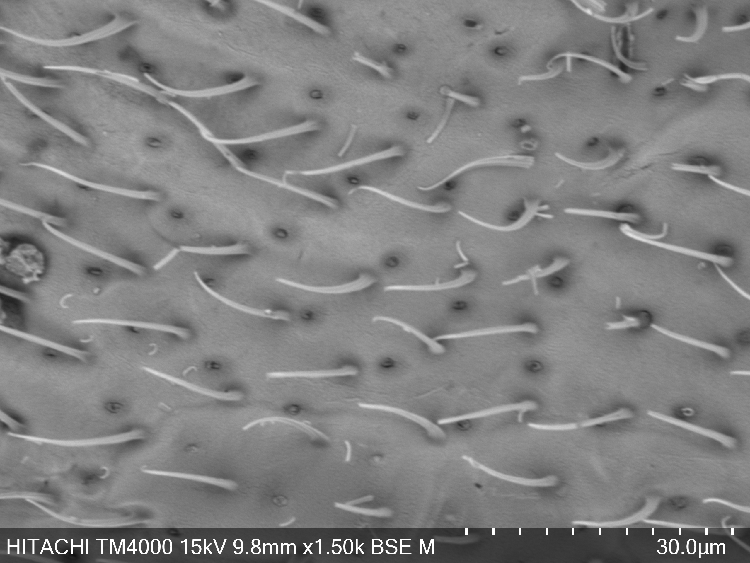
\includegraphics[scale=1]{./figs/2021-09-23-Biology_sample_002(x1.5k).pdf}
			\caption{BSE módban készült kép a biólógiai mintáról. A vékony arany bevonat ellenére (nincs Z kontraszt) kontrasztos a kép, ami azt mutatja, hogy a BSE mód is legalább kis mértékben érzékeny a minta geometriájára.}
			\label{biology1}
		\end{figure}
		\begin{figure}[H]
			\centering
			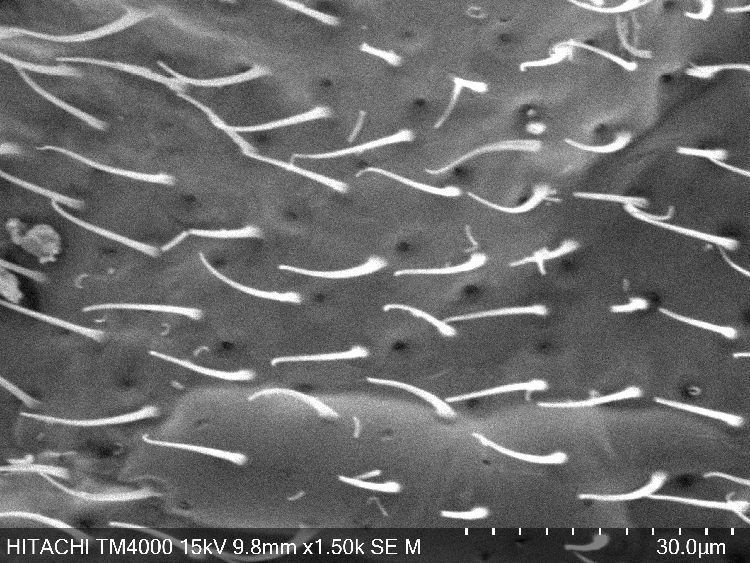
\includegraphics[scale=1]{./figs/2021-09-23-Biology_sample_003(x1.5k).pdf}
			\caption{SE módban készült kép, \aref{biology1}. képhez képest a kontraszt nagyobb. Ez így várható, hiszen az SE mód a minta geometriájára a legérzékenyebb.}
		\end{figure}
	\section{Titán minta}
		A titánból készült mintának volt egy lyukacsos része, erről készült \aref{Tiholes}. kép SE módban. Ez a kép jól illusztrálja, hogy SE módbban a geometriai információt hogyan érzékeli az elektronmikroszkóp. Lázható, hogy az üregek sötétek, ennek az az oka, hogy a kilökődő másodlagos elektronok nagy része az üreg falán landol, nem jut ki a résen, így a másodlagos elektron detektor csak kevés elektront fog detektálni. Hasonló, de kevésbé drasztikusan jelen van ez az effektus lejtők és egyéb geometriai alakzatok esetében is. 
		\begin{figure}[H]
			\centering
			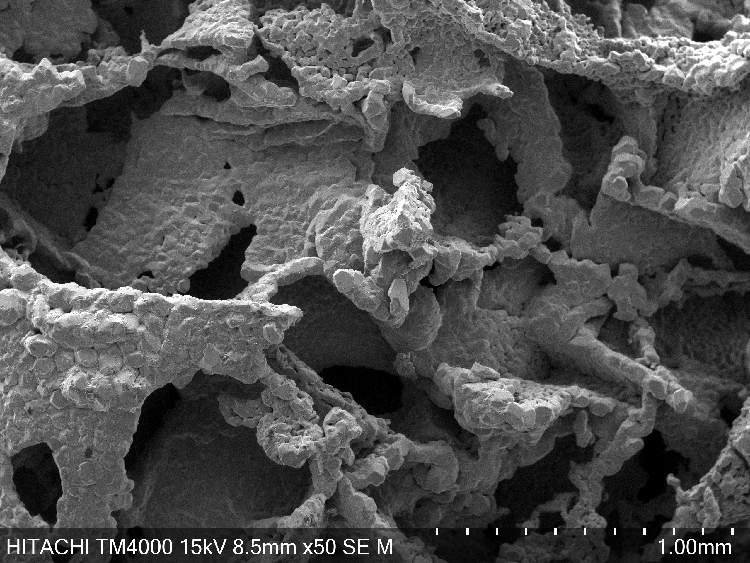
\includegraphics[scale=1]{./figs/2021-09-23-Titanium_sample_007(x50).pdf}
			\caption{SE módban készült kép a titán mintáról.}
			\label{Tiholes}
		\end{figure}
		A titán mintán a Z kontraszt is jól szemléltethető. A minta felszínén vannak kis szennyeződések, melyek a BSE módban készül \ref{tibse}. ábrán sötétebbek, mint a titán háttér. Ez arra utal, hogy a szennyeződés a titánnál kisebb rendszámú elemekből áll. \Aref{tise}. és \aref{tibse}. kép a titán minta ugyan arról a részéről készült.
		\begin{figure}[H]
			\centering
			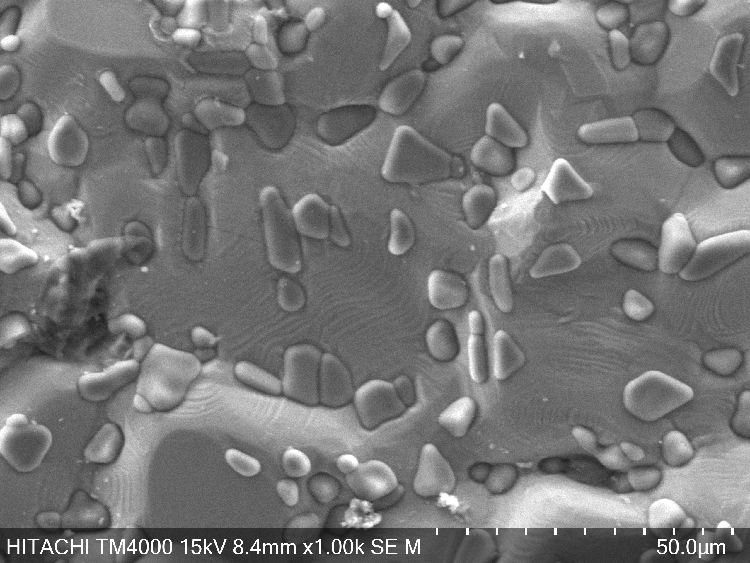
\includegraphics[scale=1]{./figs/2021-09-23-Titanium_sample_008(x1.0k).pdf}
			\caption{SE módban készült kép a titán felszíni szennyeződéseiről.}
			\label{tise}
		\end{figure}
		\begin{figure}[H]
			\centering
			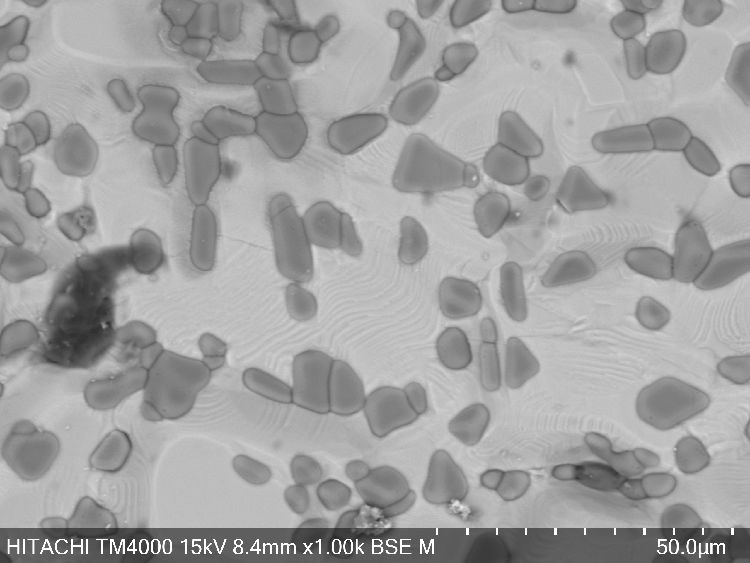
\includegraphics[scale=1]{./figs/2021-09-23-Titanium_sample_009(x1.0k).pdf}
			\caption{BSE módban készült kép a titán felszíni szennyeződéseiről.}
			\label{tibse}
		\end{figure}
		\subsection{Röntgen spektroszkópia}
			Az elektronmikroszkópban van egy beépített röntgen detektor is. A minta által kibocsátott röntgen sugarak az anyagi minőségtől függnek, és alkalmasak a minta kvalitatív vizsgálatára is. Mivel a elektronok jól fókuszáltak, az anyagi minőséget kis, a mikroszkóp felbontásának megfelelő területeken lehet vizsgálni. Két pontban végeztük el a vizsgálatot. Az első pontot az egyik BSE módban sötétnek látszó szennyeződésén vettük fel, a másodikat pedig a tiszta titán háttéren, \aref{spots}. ábrának megfelelően.
			\begin{figure}[H]
				\centering
				\includegraphics[scale=0.7]{./figs/spots.png}
				\caption{A röntgen spektrumok felvételéhez használt két pont.}
				\label{spots}
			\end{figure}
			A spektrumon a csúcsokat a mikroszkóphoz tartozó szoftver automatikusan meghatározta. A spektrum alapján titán, kalcium, és fluor volt a mintában az első pontban. Ez alapján a szennyeződés $\text{CaF}_2$ volt, a mért spektrum \aref{spectrum1}. ábrán látható. A titánra jellemző csúcsok azért detektálhatóak, mert a szennyeződés kis méret, az elektronsugár egy része áthatol rajta, és a titán mintába jut.
			\begin{figure}[H]
				\centering
				\includegraphics[scale=0.7]{./figs/spectrum1.png}
				\caption{Spectrum 1}
				\label{spectrum1}
			\end{figure}
			A második pontban felvett spektrum \aref{spectrum2}. ábrán látható. A titán az egyetlen domináns elem, ami detektálható, minden nagy detektált csúcsot megmagyaráz. Ez azt jelenti, hogy a titán minta jó közelítéssel tiszta, a kis fluorhoz tartozó csúcsot pedig a mikroszkóp felbontásánál kisebb méretű felszíni szennyeződések okozhatták, vagy akár rugalmasan szóródott elektronok, amik eltalálták a nagyobb méret szennyeződéseket.
			\begin{figure}[H]
				\centering
				\includegraphics[scale=0.7]{./figs/spectrum2.png}
				\caption{Spectrum 2}
				\label{spectrum2}
			\end{figure}
	\section{TEM rács}
		\begin{figure}[H]
			\centering
			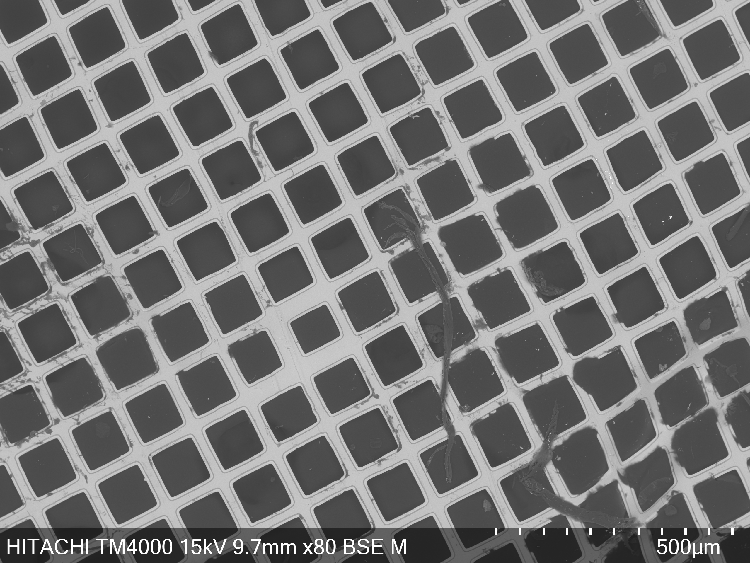
\includegraphics[scale=1]{./figs/2021-09-23-TEM_sample_006(x80).pdf}
			\caption{TEM rácsról készült BSE kép.}
			\label{temgrid}
		\end{figure}
		Az alább leírt számításokhoz tartozó Python kód megtalálható a \url{https://github.com/KurtiZoltan/SEMLabor} címen.
		
		A numpy könyvtárban található FFT függvények a következő konvenciót használják:
		\begin{equation}
			A_l = \sum_{m=0}^{n-1}a_m\exp\left\{-2\pi i\frac{ml}{n}\right\}.
			\label{fftconv}
		\end{equation}
		Az exponenciális függvény argumentumában a törtet a pixelmérettel, $D$-vel bővítve a következő tényezőket csoportosíthatjuk:
		\begin{equation}
			\begin{split}
				k_0 =& \frac{2\pi}{nD},\\
				x   =& mD,\\
				k   =& lk_0.
			\end{split}
		\end{equation}
		Ezekkel a jelölésekkel \aeqref{fftconv} egyenlet alakja
		\begin{equation}
			A_l = \sum_x a(x)\exp\left\{-ilk_0x\right\},
		\end{equation}
		tehát a fourier transzformált képen egy pixelhez tartozó hullámszám vektor változás a $k_0$. Ez azt jelenti, hogy a TEM rácsról készült kép esetében az $x$ és $y$ irányokban a pixelekhez különböző $k_0$ tartozik. Amennyiben a TEM rács nem párhuzamos az $x$ és $y$ irányokkal, az egy dimenziós fourier spektrumon található csúcs távolságának meghatározásában ezt a különbséget figyelembe kell venni. Hogy demonstráljam a programom helyességét, azt a képet választottam, ahol a rács ferdén áll, és két különböző irány mentén lemértem az első csúcs távolságát. Amennyiben a program helyesen működik, a két irányban mért periódus megegyezik, mivel a háló négyzetrácsos.
		\begin{figure}[H]
			\centering
			\includegraphics[scale=1]{./figs/2dfft.pdf}
			\caption{\Aref{temgrid}. kép kétdimenziós diszkrét Fourier-transzformáltja. Az ábrázolhatóság kedvéért az ábrán a spektrum abszolútérték négyzetét ábrázoltam logaritmikus skálán.}
			\label{2dfft}
		\end{figure}
		\begin{figure}[H]
			\centering
			\includegraphics[scale=1]{./figs/fftlines.pdf}]
			\caption{\Aref{2dfft}. ábra középpontja kinagyítva. \Aref{temgrid}. ábrán látható rácshoz tartozó irányokra a középponton áthaladó szakaszokat illesztettem a meredekség megbecsülésével.}
			\label{fftlines}
		\end{figure}
		\begin{figure}[H]
			\centering
			\includegraphics[scale=1]{./figs/1dpsd.pdf}
			\caption{\Aref{fftlines}. ábrán látható piros és kék irányokhoz tartozó spektrum abszolútérték négyzete, logaritmikus skálán, a narancssárga függőleges vonalak a periódushoz tartozó hullámszám egész számú többszörösei.}
			\label{1dpsd}
		\end{figure}
	\bibliographystyle{abeld}
    \bibliography{tex/ref}
\end{document}











